\begin{enumerate}[label=\thesection.\arabic*.,ref=\thesection.\theenumi]

\item
 The open-loop transfer function of a plant in a unity feedback configuration is given as 
\begin{equation}
    G\brak{s} = \frac{K(s+4)}{(s+8)(s^{2}-9)}
\end{equation}
 The value of the gain $K(>0)$ for which $-1 + \j2$ lies on the root locus is
    
  

\solution
  The closed loop transfer function for a negative feed back system is:
  \begin{equation}
      F\brak{s} = \frac{G\brak{s}}{1+G\brak{s}H\brak{s}}
  \end{equation}
Since it is a unity feed back system, $H\brak{s} = 1$, and now using the characteristic equation at $s_{1} = -1 + \j2$
\begin{equation}
1 + G\brak{s_{1}}H\brak{s_{1}} = 0
\end{equation}
\begin{equation}
 G\brak{s_{1}} = -1
\end{equation}
\begin{equation}
 \abs{G\brak{s_{1}}} = 1
\end{equation}


\begin{equation}
    G\brak{s_{1}} = \frac{K(s_{1}+4)}{(s_{1}+8)(s_{1}^{2}-9)}
\end{equation}
\begin{equation}
    G\brak{s_{1}} = \frac{K(s_{1}+4)}{(s_{1}+8)(s_{1}+3)(s_{1}-3)}
\end{equation}
\begin{equation}
    G\brak{s_{1}} = \frac{K(3+\j2)}{(7+\j2)(2+\j2)(-4+\j2)}
\end{equation}
\begin{equation}
    \abs{G\brak{s_{1}}} = \frac{K\sqrt{13}}{\sqrt{51}\sqrt{8}\sqrt{20}} = 1
\end{equation}
\begin{equation}
    K = 25.05
\end{equation}


\begin{equation}
    F\brak{s} = \frac{25.05(s+4)}{s^{3}+8s^{2}+16.05s+28.2}
\end{equation}

    $Z_{1}=-4, P_{1}=-6.13, P_{2}=-0.93+\j1.93, P_{3}=-0.93-\j1.93$


\begin{figure}
\centering
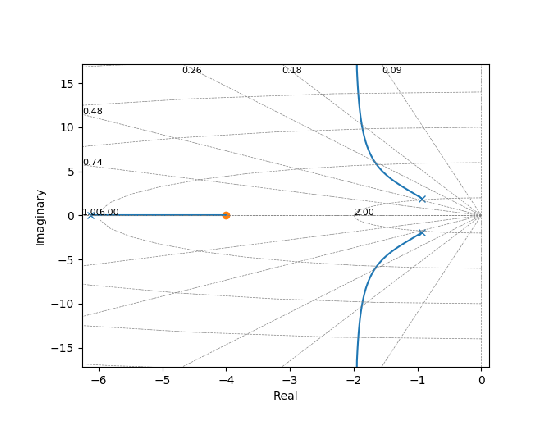
\includegraphics[width=\columnwidth]{figs/ee18btech11052.eps}
\caption{Root locus plot for verification}
\end{figure}


\begin{lstlisting}
codes/ee18btech11052.py
\end{lstlisting}
    
\end{enumerate}

